\documentclass{scrartcl}
\usepackage{physics}   % Matrixes and Dirac-notation
\usepackage{amsmath}   % Binear equations
\usepackage{booktabs}  % Tabs
\usepackage{graphicx}  % Pictures/figures
\usepackage{listings}  % Source code
\usepackage{color}     % Colors
\usepackage{float}
\usepackage{hyperref}

\definecolor{dkgreen}{rgb}{0,0.6,0}
\definecolor{gray}{rgb}{0.5,0.5,0.5}
\definecolor{mauve}{rgb}{0.58,0,0.82}

%Defining source code
\lstset{frame=tb,
  language=Python,
  aboveskip=3mm,
  belowskip=3mm,
  showstringspaces=false,
  columns=flexible,
  basicstyle={\small\ttfamily},
  numbers=none,
  numberstyle=\tiny\color{gray},
  keywordstyle=\color{blue},
  commentstyle=\color{dkgreen},
  stringstyle=\color{mauve},
  breaklines=true,
  breakatwhitespace=true,
  tabsize=3
}
\begin{document}
\begin{titlepage}
	\centering
	{\scshape\LARGE $\star\star\star$  \par}
	\vspace{4cm}
	{\scshape\huge FYS2160 - Thermal Physics  \par}
	\vspace{1cm}
	{\scshape\Large Oblig 03\par}
	\vspace{2cm}
	{\Large\itshape Even Marius Nordhagen\par}
	\vfill
	{\large \today\par}
\end{titlepage}

\section*{Exercises}
The aim of this project is to use thermal dynamic units in practice, which is done by working with physical systems with various number of particles, $N$. 

For a van der Waals gas, the Hermholtz free energy is given by
\begin{equation}
F_{wdW}=-NkT\Bigg(\ln\bigg(\frac{n_Q(V-Nb)}{N}\bigg)+1\Bigg)-\frac{aN^2}{V}
\end{equation}

\subsection*{a)}
In general the pressure is given by
\begin{equation}
p=-\bigg(\frac{\partial F}{\partial V}\bigg)_{T,N}
\end{equation}
so for the van der Waals gas we have the pressure
\begin{equation}
p=NkT\bigg(\frac{N}{n_Q(V-Nb)}\bigg)\cdot \frac{n_Q}{N}-\frac{aN^2}{V^2}=\frac{NkT}{V-Nb}-\frac{aN^2}{V^2}
\label{eq:pressure}
\end{equation}
This is called the \textit{Equation state of the van der Waals system}.

\subsection*{b)}
Via the relation $\hat{p}=p/p_c$, we can use the expression we found in the first exercise.
\begin{equation}
\hat{p}=\frac{1}{p_c}\bigg(\frac{NkT}{V-Nb}-\frac{aN^2}{V^2}\bigg)
\label{eq:p(V)}
\end{equation}
We want to replace all the quantities with dimensionless quantities, and for that we can use the relations
\begin{itemize}
\item $V=\hat{V}V_c=3Nb\hat{V}$
\item $T=\hat{T}T_c=\frac{8a}{k27b^2}\hat{T}$
\item $p_c=\frac{a}{27b^2}$
\end{itemize}
\begin{equation}
\hat{p}=\frac{27b^2}{a}\bigg(\frac{(8a/27b)\hat{T}}{3b\hat{V}-b}-\frac{aN^2}{(3Nb\hat{V})^2}\bigg)=\frac{8\hat{T}}{3\hat{V}-1}-\frac{3}{\hat{V}^2}
\end{equation}
This is called the \textit{The law of Corresponding states}. 

\subsection*{c)}
In this exercise I was asked to plot the behaviour of the van der Waals gas for $T/T_c\in[0.4,20]$. The plot can be found in Figure (\ref{fig:behav}).
\begin{figure}[H]
\centering
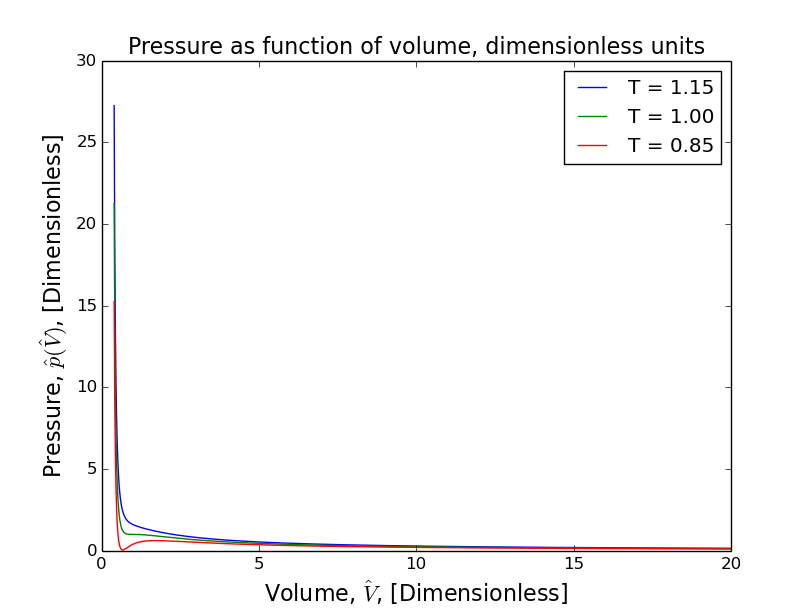
\includegraphics[width=120mm]{oblig3_1.png}
\caption{Pressure as a function of volume $\hat{V}$ when $\hat{V}\in[1/2.0, 1/0.2]$ plotted for $\hat{T}=[0.85, 1.00, 1.15]$ with dimensionless units.}
\label{fig:behav}
\end{figure}
In my option I think it would be reasonable to zoom into the first part of the plot to study the exact behaviour of the graphs. Then we would see that a given pressure provides multiple possible volumes for $\hat{T}=0.85$. When $\hat{T}=1.0$ the damping is critical, so we can assume that we will have multiple possible volumes for a given pressure for all $\hat{T}<1.0$, (which corresponds to $T/T_c<1.0$). $T_c$ is the so-called critical temperature, which makes sense. Another thing we would see, is that the pressure increases for increasing volumes, which is obviously an unphysical situation. The ideal gas law states that $pV=nRT$ where all the parameters on the right hand side are constants (in our case). Then both the pressure and volume cannot increase in the same time! We can conclude that all $\hat{T}<1.0$ are unphysical isotherms. \newline\textit{The program can be found in Appendix A}

\subsection*{d)}
By using the relation $\hat{V}=1/\hat{\rho}$, we find that
\begin{equation}
\hat{p}=\frac{8\hat{T}}{3/\hat{\rho}-1}-\frac{3}{1/\hat{\rho}^2}=\frac{8\hat{\rho}\hat{T}}{3-\hat{\rho}}-3\hat{\rho}^2
\end{equation}

\subsection*{e)}
\begin{figure}[H]
\centering
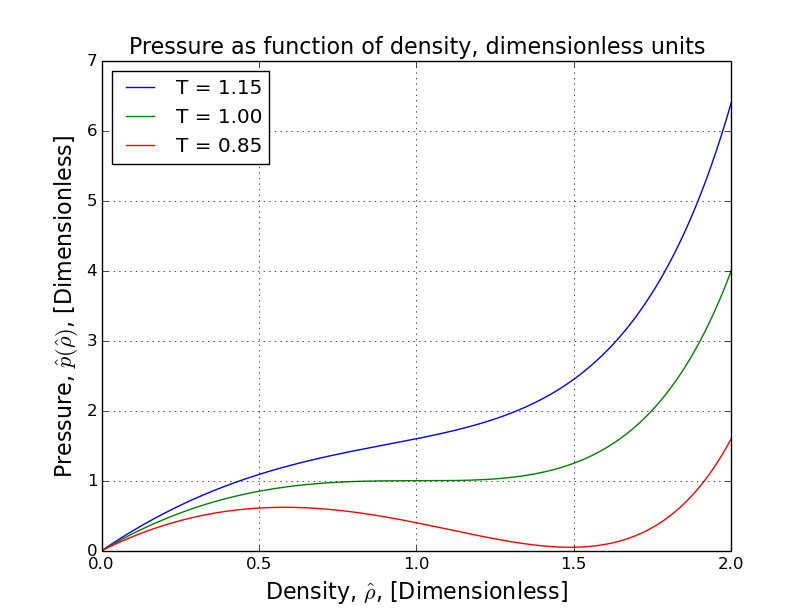
\includegraphics[width=120mm]{oblig3_2.png}
\caption{Pressure as a function of density $\hat{\rho}$ when $\hat{\rho}\in[0.2, 2.0]$ plotted for $\hat{T}=[0.85, 1.00, 1.15]$ with dimensionless units.}
\label{fig:e}
\end{figure}
\textit{The program can be found in Appendix B}

\subsection*{f)}
From Figure (\ref{fig:e}) we can see that for $\hat{T}=1.15$ and $\hat{T}=1.0$ the functions are monotonic (are growing in the whole interval), but this does not apply for the case then $\hat{T}=0.85$. In that case, the pressure is sinking about $\hat{\rho}=1$, which means that the density become non-unique function of pressure since one pressure value corresponds to multiple values of density. This also means that we cannot express density as function of pressure, because a function is uniquely determined. 

\subsection*{g)}
The isothermal compressibility is defined by
\begin{equation}
\kappa=\frac{1}{\rho}\bigg(\frac{\partial\rho}{\partial p}\bigg)
\end{equation}
which is negative when $\rho(p)$ is decreasing. We do not have this function, but in Figure (\ref{fig:e}) we have a plot of $p(\rho)$, and $\Big(\frac{\partial p}{\partial\rho}\Big)$ will be negative in the same interval as $\Big(\frac{\partial\rho}{\partial p}\Big)$. We can see that the isothermal compressibility is negative for $\hat{T}=0.85$ in the interval $\hat{\rho}\in[0.5,1.5]$, which is an unphysical situation. In the same way we can see that the $\hat{T}$-graph has a saddle point, so again we can conclude that $\hat{T}<1.0$ are unphysical quantities.

\subsection*{h)}
Gibbs free energy is defined by
\begin{equation*}
G=F-V\bigg(\frac{\partial F}{\partial V}\bigg)_{T,N}=F+pV.
\end{equation*}
$p$ is expressed in exercise $a)$, and we have $F$ from the project description. 
\begin{equation*}
G=pV+F=\frac{NVkT}{V-Nb}-\frac{aN^2}{V}-NkT\Bigg(\ln\bigg(\frac{n_Q(V-Nb)}{N}\bigg)+1\Bigg)-\frac{aN^2}{V}
\end{equation*}
\begin{equation}
=\frac{NVkT}{V-Nb}-\frac{2aN^2}{V}-NkT\Bigg(\ln\bigg(\frac{n_Q(V-Nb)}{N}\bigg)+1\Bigg)
\label{eq:G(T,V,N)}
\end{equation}

\subsection*{i)}
The clue to solve this exercise is the $c(T)$ function, which is a function of temperature alone. I will use the expression from the previous exercise. From Equation (\ref{eq:pressure}) we have that
\begin{equation*}
\frac{aN^2}{V}=\frac{BkTV}{V-Nb}-pV
\end{equation*}
By inserting this into Equation (\ref{eq:G(T,V,N)}) we find that
\begin{equation*}
G=\frac{NVkT}{V-Nb}-\frac{aN^2}{V}-\frac{NVkT}{V-Nb}+pV-NkT\Bigg(\ln\bigg(\frac{n_Q(V-Nb)}{N}\bigg)+1\Bigg)
\end{equation*}
Two of the terms cancel, and the logarithm can be separated:
\begin{equation*}
=-\frac{aN^2}{V}+pV-NkT\Bigg(\ln\bigg(\frac{n_Q}{N}\bigg)+\ln(V-Nb)+1\Bigg)
\end{equation*}
\begin{equation}
=-NkT\ln(V-Nb)-\frac{aN^2}{V}+pV+NkTc(T)
\end{equation}
where 
\begin{equation*}
c(T)=\ln\bigg(\frac{n_Q(T)}{N}\bigg)+1
\end{equation*}

\subsection*{j)}
I will start with the expression from the previous exercise, and use that $\hat{g}=\frac{8G}{3NkT_c}$ and $T=\hat{T}T_c$.
\begin{equation*}
\hat{g}=-\frac{8\hat{T}}{3}\ln(V-Nb)-\frac{8Na}{3kT_c}\frac{1}{V}+\frac{8pV}{3NkT_c}+\frac{8}{3}\hat{T}c(T)
\end{equation*}
The last term does not depend on the pressure or density, so we can ignore this. To simplify the expression further, I will use
\begin{equation*}
V=\hat{V}V_c=3Nb\hat{V}=\frac{3Nb}{\hat{\rho}}
\end{equation*}
The first term can be written as
\begin{equation*}
\frac{8\hat{T}}{3}\ln(V-Nb)=\frac{8\hat{T}}{3}\ln\Bigg(Nb\bigg(\frac{3}{\hat{\rho}}-1\bigg)\Bigg)=\frac{8\hat{T}}{3}\Bigg(\ln Nb+ln\bigg(\frac{3}{\hat{\rho}}-1\bigg)\Bigg)=\frac{8\hat{T}}{3}\Bigg(\ln\bigg(\frac{3}{\hat{\rho}}-1\bigg)\Bigg)
\end{equation*}
Where I again ignored a term which does not depend on the pressure or density. The second term can be written as
\begin{equation*}
\frac{8aN^2}{3NkT_c}\frac{\hat{\rho}}{3Nb}=\frac{8a27bN^2\hat{\rho}}{8a9bN^2}=3\hat{\rho}
\end{equation*}
For the last term, we also need the relation
\begin{equation*}
p=\hat{p}p_c=\hat{p}\cdot \frac{a}{27b^2}
\end{equation*}
we get
\begin{equation*}
\frac{8pV}{3NkT_c}=\frac{8\hat{p}3Nb27ba}{8a3N\hat{\rho}27b^2}=\frac{\hat{p}}{\hat{\rho}}
\end{equation*}
We end up with 
\begin{equation}
\hat{g}=-3\hat{\rho}-\frac{8\hat{T}}{3}\Bigg(\ln\bigg(\frac{3}{\hat{\rho}}-1\bigg)\Bigg)+\frac{\hat{p}}{\hat{\rho}}
\end{equation}

\subsection*{k)}
For plotting pressure as function of density, I used Equation (\ref{eq:p(V)}). For the next plot I needed to use the relation $\hat{V}=1/\hat{\rho}$, and plotted $\hat{p}(\hat{V})$ on the x-axis and $\hat{V}$ on the y-axis. For the last plot, I again used $\hat{V}=1/\hat{\rho}$ to express $\hat{g}$ as function of $\hat{V}$ (and $\hat{p}$), and plotted $\hat{p}(\hat{V}$ on the x-axis with the same $\hat{V}$-values as for $\hat{g}$. The plot can be found in Figure (\ref{fig:k1}).
\begin{figure}[H]
\centering
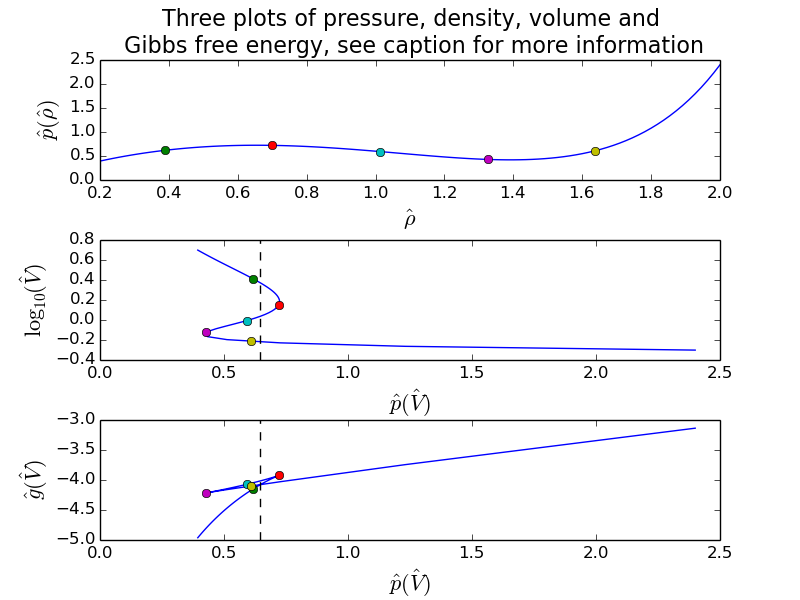
\includegraphics[width=150mm]{oblig3_3.png}
\caption{The first subplot shows pressure as function of density, with several highlighted point which are marked periodically. The second subplot shows pressure as function of volume, with the same highlighted points as from the first one. The last subplot presents Gibbs free energy as function of pressure, where still the same highlighted points are included. This plot is further discussed in the text, where the two others are retracted. All the variables are dimensionless.}
\label{fig:k1}
\end{figure}
The Gibbs free energy could been plotted as a function of volume, but it's more powerful to plot it as a function of the pressure, which the latest subplot in Figure (\ref{fig:k1}) shows. I decided to make a new, zoomed version of the latest subplot to be able to see the details, see Figure (\ref{fig:k2}).
\begin{figure}[H]
\centering
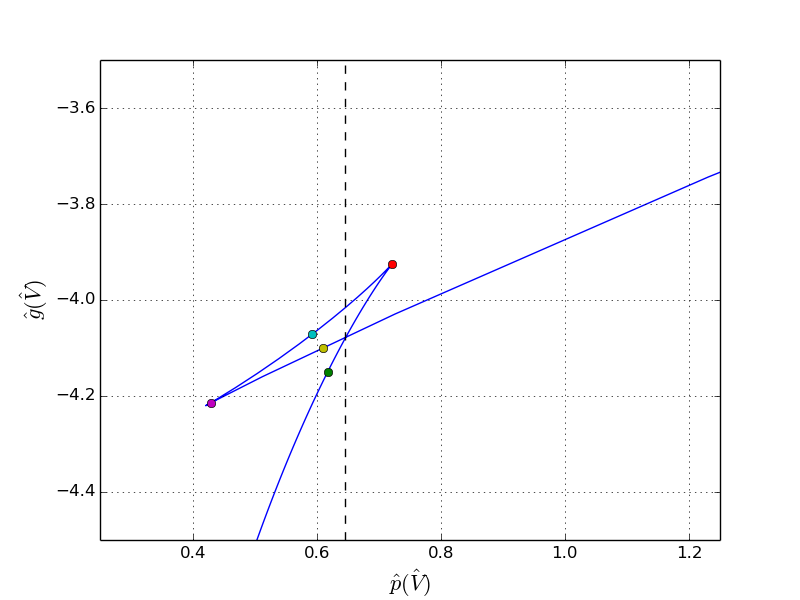
\includegraphics[width=150mm]{oblig3_4.png}
\caption{Gibbs free energy plotted as a function of pressure. Both the variables are dimensionless.}
\label{fig:k2}
\end{figure}
As we can see, the graph takes a "loop", which means that it intersects itself. A vertical dashed line is drawn through the point where the the graph starts self intersect (I will call it the intersection point). 
\newline\textit{The program can be found in Appendix C}

\subsection*{l)}
The thermodynamically stable state is where the Gibbs free energy is minimized, so we can find the minimum of Gibbs free energy if we know the transition from a gas to a liquid. The definition of a gas is that the volume is decreasing rapidly when we are increasing the pressure. As we can see from the second subplot in Figure (\ref{fig:k}), this is the situation until the pressure has reached the green point (circa). The latest subplot tells us that the red, cyan, purple and yellow points are unphysical (the loop is not a physical situation), and as the pressure is decreasing, the system will go straight from the intersection point and to the right on the lower part of the curve (it will not follow the loop). After this point the volume is decreasing slowly when the pressure is increasing, so here fluid has been transformed into a liquid. This means that the intersection point is where the state is thermodynamically stable, and therefore where the Gibbs free energy is minimized. 

\subsection*{m)}
In this exercise I'm supposed to find the exact indices of the intersection point, so far I've just found the x-index of the point by looking at the graph. There is a pre-built program in MATLAB that is doing this\footnote{\url{https://se.mathworks.com/matlabcentral/fileexchange/13351-fast-and-robust-self-intersections/content/selfintersect.m}}, so this time I will use that language. The result is that the intersection point is located at the indices $p_0=0.647$ and $g_0=-4.0763$ (when I'm running the program with $N=1000$ time steps), and we can see that the x-index which I found graphic ($p_0=0.645$) was not fully correct. When drawing a (dashed) vertical line at $p=0.647$ together with $V(p)$ and $\rho(p)$, we get the two plots in Figure (\ref{fig:m1}) and (\ref{fig:m2}).
\begin{figure}[H]
\centering
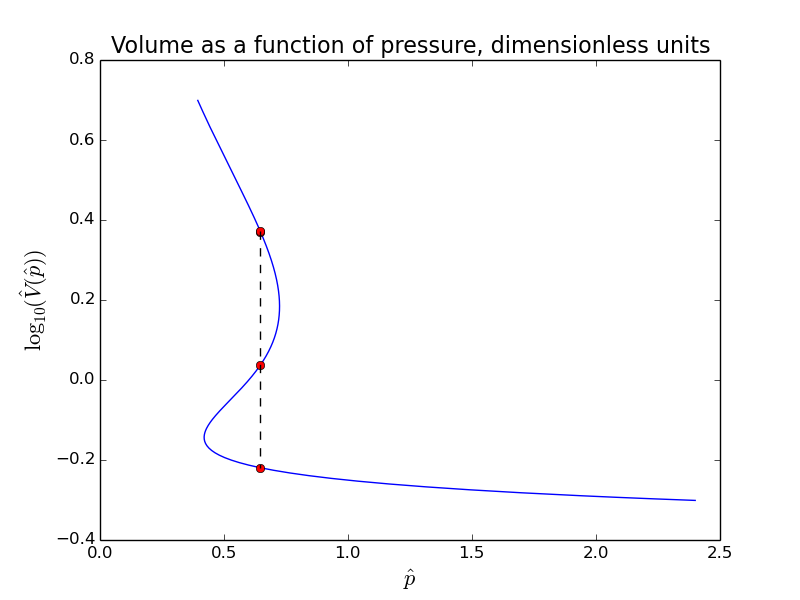
\includegraphics[width=120mm]{oblig3_5.png}
\caption{Volume as a function of pressure with a line drawn between the points where the pressure is $p_0=0.647$. The parameters are dimensionless.}
\label{fig:m1}
\end{figure}
\begin{figure}[H]
\centering
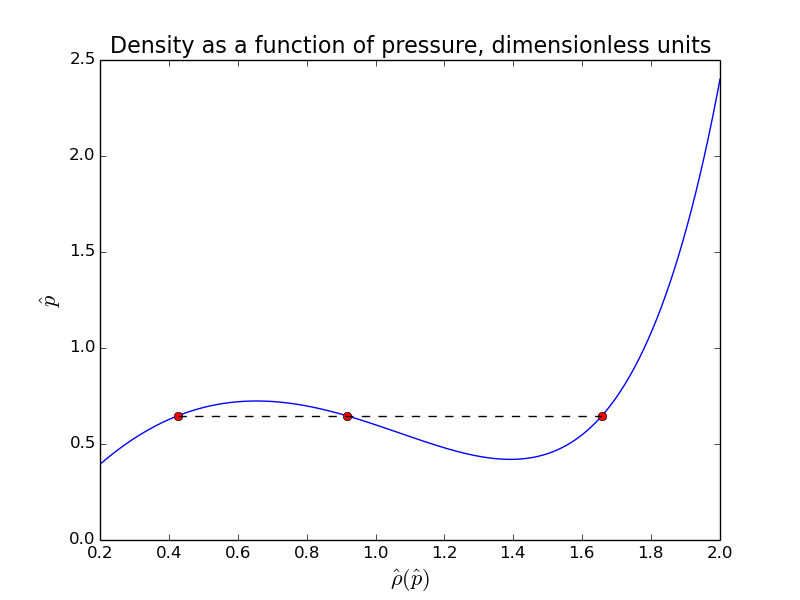
\includegraphics[width=120mm]{oblig3_6.png}
\caption{Density as a function of pressure with a line drawn between the points where the pressure is $p_0=0.647$. The parameters are dimensionless.}
\label{fig:m2}
\end{figure}
Here I first found when the graphs where equal to $p_0=0.647$, and then I plotted (dashed) lines between them. In both cases we can see that the line segment is making two "areas" with the curves, and in the first case the areas are actually equal! It does not looks like this because I've plotted the logarithm of the volume, but it really makes sense cause the two "integrals" (areas) cancel. As I earlier mentioned, the line segment spans out the area that corresponds to the unphysical states, something that is discussed further in the next exercise. 
\newline\textit{Even though the exact indices of the intersection point are found in MATLAB, the plots in this exercise are made by Python. The MATLAB script which calls on selfintersect.m is found in Appendix D, while the python program which makes the plots above is found in Appendix E.}

\subsection*{n)}
Between the intersections we have phase equilibrium, where we have both liquid and gas, which is unphysical (as we have seen). In general we will have a phase diagram like in Figure (\ref{fig:n}).
\begin{figure}[H]
\centering
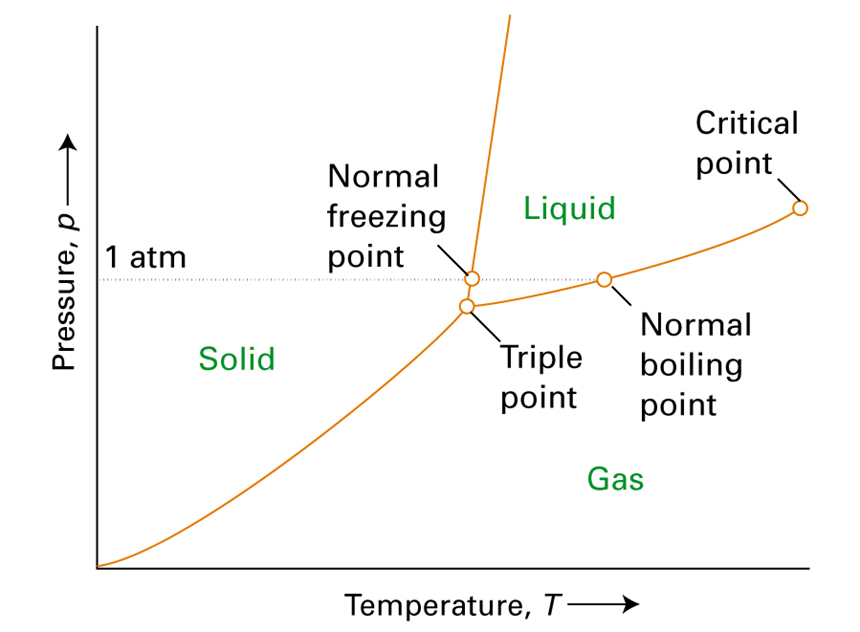
\includegraphics[width=150mm]{graph2.png}
\caption{Phase diagram for a substance (in this case water). The figure is downloaded from \url{ http://1.bp.blogspot.com/-2vz5W8D2QRI/UINm3lFHaGI/AAAAAAAAAEY/4Hp9VmrbTIM/s1600/graph2.png}}
\label{fig:n}
\end{figure}
We can see that this is a little similar to the plot we have for Gibbs free energy, so it seems like the system first is going further toward the gas state after the intersection point, but then change its mind and going to the liquid state. I guess this happens when most of the particles are in the liquid state.

\subsection*{o)}
In this exercise we are studying how the volume as a function of pressure behaviours for different temperatures. In Figure (\ref{fig:o}) this function of plotted for $\hat{V}\in[1/2.0, 1/0.2]$ and with the four temperatures $\hat{T}=[0.85, 0.90, 0.95, 1.00]$. 
\begin{figure}[H]
\centering
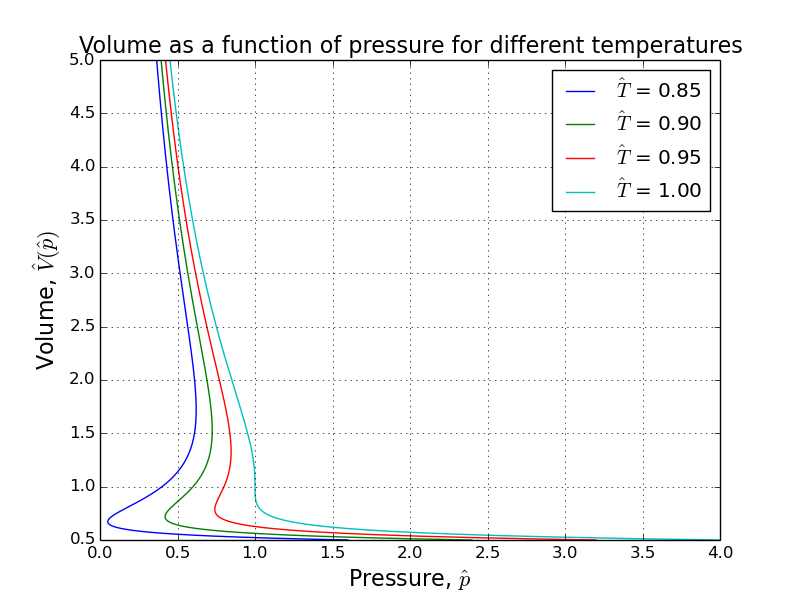
\includegraphics[width=150mm]{oblig3_7.png}
\caption{Volume as function of pressure plotted for $\hat{V}\in[1/2.0, 1/0.2]$ and with the four temperatures $\hat{T}=[0.85, 0.90, 0.95, 1.00]$. All parameters are dimensionless.}
\label{fig:o}
\end{figure}
We can see that $\hat{p}(\hat{V})$ is a non-unique function when $\hat{T}<1.0$, but for $\hat{T}=1.00$ the function is unique since a value of volume corresponds to one single value of pressure. This is exactly what we saw in exercise f), but we can get the same result with the same approach as for the last few exercises. We have seen that we have some critical points (which separates the physical and the unphysical states), and we can imagine that these points are coming closer for higher temperatures by looking at Figure (\ref{fig:o}). For $\hat{T}=1.00$ all the points will be on the same indices, which means that we do not have  unphysical states anymore. We can conclude that $\hat{T}$ is the critical temperature limit, that is $T/T_c$. If $T\ge T_c$, we will not have phase transition and therefore not unphysical states (when we are studying the phenomena this way), but for $T<T_c$ we will have some unphysical states for this model. 
\newline\textit{The program is found in Appendix F}
\newpage
\section*{Code attachment}
\subsection*{Appendix A}
\lstinputlisting[language=Python]{oblig3_c.py}
\subsection*{Appendix B}
\lstinputlisting[language=Python]{oblig3_e.py}
\subsection*{Appendix C}
\lstinputlisting[language=Python]{oblig3_k.py}
\subsection*{Appendix D}
\lstinputlisting[language=MATLAB]{FYS2160_oblig3.m}
\subsection*{Appendix E}
\lstinputlisting[language=Python]{oblig3_m.py}
\subsection*{Appendix F}
\lstinputlisting[language=Python]{oblig3_o.py}
\end{document}